\chapter{Euler Paths/Cycles}

Ajur was tired after listening to a lot of definitions and examples. He complained to Jura that looked too much like a Math class and he preferred fun Math problems instead. As Ajur was mentioning, Rishnak was overhearing this conversation. Rishnak too felt that the pprvious day's conversation was very cut and dry. His ghost friends were accusing of making the beautiful subject of Graph Theory dull and monotnous.


An Euler walk of a connected graph is a walk that includes every edge exactly once. If the starting vertex and the ending vertex are the same then it is called a closed Euler walk. Of course the name Euler comes from 
Rishnak decided to take on the oldest problem on Graph Theory Euler walk and closed Euler walk. Rishnak caught up with Ajur and Jura walking along a desolate road. Rishnak asked Ajur in the Figure \ref{4g1} whether there is a walk starting from vertex 2 to vertex 4 passing all the edges exactly once [This is what is known as an Eulerian walk]. Ajur saw there is a cycle (2,3,4,1,2). After this cycle, there is just one edge (2,4) left. Hence Ajur constructed an Eulerian walk by combining the two as (2,(2,3),3,(3,4),4,(4,1),1,(1,2),2,(2,4),4) or written simply as (2,3,4,1,2,3) by omitting the edges. Ajur illustrated this Figure \ref{4g15} Ajur further added that there is no closed Eulerian walk as that would imply that the edges have to be split into cycles (with no edges in common among the cycles). This will mean that the degrees of every vertex has to be even. Rishnak was much impressed with Ajur's reasoning. 


\begin{figure}
\begin{center}
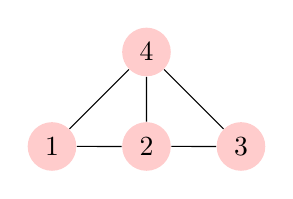
\begin{tikzpicture}
  [scale=.6,auto=left,every node/.style={circle,fill=red!20}]
  \node (n1) at (1,7) {1};
  \node (n2) at (3,7)  {2};
  \node (n3) at (5,7)  {3};
  \node (n4) at (3,9)  {4};

  \foreach \from/\to in {n1/n2,n2/n3,n2/n4,n1/n4,n3/n4}
    \draw (\from) -- (\to);

\end{tikzpicture}
\caption{ Example Graph with 4 vertices and 5 edges}\label{4g1}
\end{center}
\end{figure}

\begin{figure}
\begin{center}
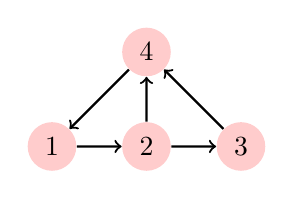
\begin{tikzpicture}
  [scale=.6,auto=left,every node/.style={circle,fill=red!20}]
  \node (n1) at (1,7) {1};
  \node (n2) at (3,7)  {2};
  \node (n3) at (5,7)  {3};
  \node (n4) at (3,9)  {4};

\path [->,draw,thick]
(n2) edge  (n3)
(n3) edge   (n4)
(n4) edge   (n1)
(n1) edge   (n2)
(n2) edge  (n4)
;
\end{tikzpicture}
\caption{ Eulerian Path from vertex 2 to vertex 4 2-3-4-1-2-4 of Figure \ref{4g1}}\label{4g15}
\end{center}
\end{figure}
\vspace{2cm}
Rishnak then asked Ajur whether you can start a walk from vertex 1 to vertex 9 and visit all edges once and only once (Eulerian walk from vertex 1 to vertex 9) in connected graph in Figure \ref{4g2}.
Ajur was perplexed. Then he tried to reason - he can break them into cycles. (2,3,7),(7,6,5,4), (3,4,8)  - None of these cycles had any edge in common. So he constructed a 
walk as (1,(1,2),2,(2,3),3,(3,4),4,(4,8),8,(8,3),3,(3,7),7, (7,6),6,(6,5),5,(5,4).4,(4,7),7,(7,2),2,(2,8),8,(8,9),9). Ajur further explained that he obtained this Eulerian walk by essentially by combining these cycles. He illustrated his walk in \ref{4g25}. Ajur responded that there is no closed Eulerian walk in this graph \ref{4g2} as all the vertices are not of even degree.

\begin{figure}
\begin{center}
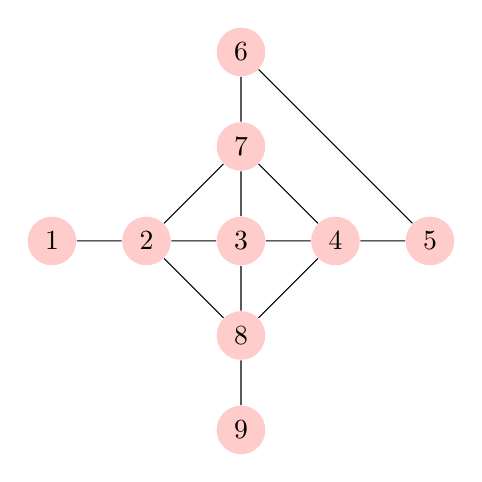
\begin{tikzpicture}
  [scale=.6,auto=left,every node/.style={circle,fill=red!20}]
  \node (n1) at (1,7) {1};
  \node (n2) at (3,7)  {2};
  \node (n3) at (5,7)  {3};
  \node (n4) at (7,7) {4};
  \node (n5) at (9,7)  {5};
  \node (n6) at (5,11)  {6};
   \node (n7) at (5,9) {7};
   \node (n8) at (5,5) {8};
   \node (n9)  at (5,3) {9};
  \foreach \from/\to in {n1/n2,n2/n3,n3/n4,n4/n5,n6/n7,n7/n3,n3/n8,n8/n9,n2/n7,
  n4/n7,n4/n8,n8/n2,n6/n5}
    \draw (\from) -- (\to);

\end{tikzpicture}
\caption{ Example Graph with 9 vertices and 13 edges}\label{4g2}
\end{center}
\end{figure}

\begin{figure}
\begin{center}
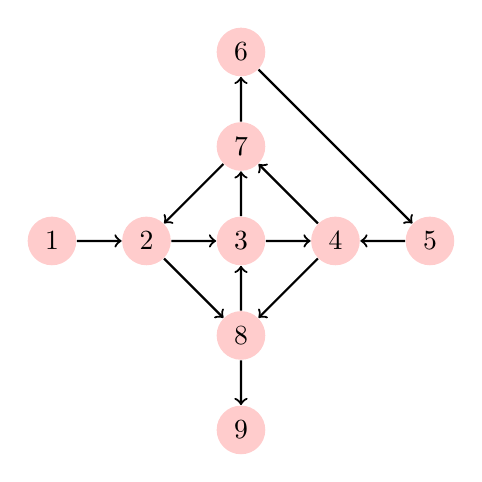
\begin{tikzpicture}
  [scale=.6,auto=left,every node/.style={circle,fill=red!20}]
  \node (n1) at (1,7) {1};
  \node (n2) at (3,7)  {2};
  \node (n3) at (5,7)  {3};
  \node (n4) at (7,7) {4};
  \node (n5) at (9,7)  {5};
  \node (n6) at (5,11)  {6};
   \node (n7) at (5,9) {7};
   \node (n8) at (5,5) {8};
   \node (n9)  at (5,3) {9};
 \path [->,draw,thick] 
  (n1) edge  (n2)
  (n2) edge (n3)
  (n3) edge (n4)
  (n4) edge (n8)
  (n8) edge (n3)
  (n3) edge (n7)
  (n7) edge (n6)
  (n6) edge (n5)
  (n5) edge (n4)
  (n4) edge (n7)
  (n7) edge (n2)
  (n2) edge (n8)
  (n8) edge (n9)
;
\end{tikzpicture}
\caption{ Eulerian Walk from vertex 1 to vertex 9  1-2-3-4-8-3-7-6-5-4-7-2-8-9 of Figure \ref{4g2}}\label{4g25}
\end{center}
\end{figure}

\vspace{3in}
Rishnak asked Ajur how would you make the graph shown in Figure \ref{4g2} to have a closed Eulerian Walk. Ajur reasoned that there are exactly two vertices of odd degrees, namely, vertices 1 and 9. If we join an edge between 1 and 9,  every vertex will have an even degree and hence a closed Eulerian Walk and that walk will be 1-2-3-4--8--7-6-5-4-7-2-8-9-1. Ajur also drew a graph.

\begin{figure}
\begin{center}
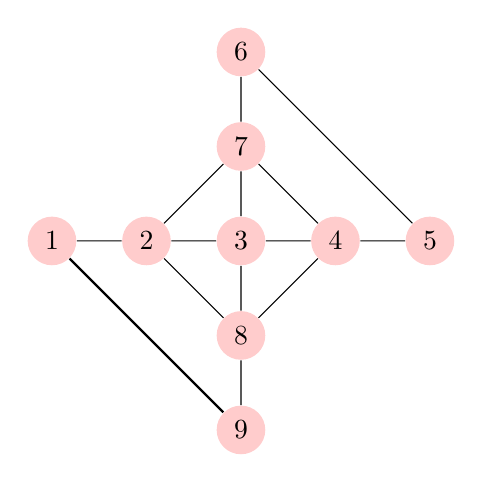
\begin{tikzpicture}
  [scale=.6,auto=left,every node/.style={circle,fill=red!20}]
  \node (n1) at (1,7) {1};
  \node (n2) at (3,7)  {2};
  \node (n3) at (5,7)  {3};
  \node (n4) at (7,7) {4};
  \node (n5) at (9,7)  {5};
  \node (n6) at (5,11)  {6};
   \node (n7) at (5,9) {7};
   \node (n8) at (5,5) {8};
   \node (n9)  at (5,3) {9};
  \foreach \from/\to in {n1/n2,n2/n3,n3/n4,n4/n5,n6/n7,n7/n3,n3/n8,n8/n9,n2/n7,
  n4/n7,n4/n8,n8/n2,n6/n5}
    \draw (\from) -- (\to);
\path[thick] (n1) edge (n9);
\end{tikzpicture}
\caption{ Closed Eulerian Walk with edge (1,9) added to Figure \ref{4g2}}\label{4g255}
\end{center}
\end{figure}

Rishnak asked how will you make graph shown in Figure \ref{4g1} to have a closed Eulerian walk. Ajur now had problem. The two vertices which have odd degrees 2 and 4, have an already an edge between them. However, he remembered the definition of a multigraph, where in between any two vertices, there can be more than one edge. So he added another edge between 2 and 4 and there is a closed Eulerian walk 2-3-4-1-2-4-2. Ajur again drew a graph as shown in Figure \ref{4g155}
Ajur added that if a graph is not connected, there is neither Eulerian walk nor a closed Eulerian walk.
\begin{figure}
\begin{center}
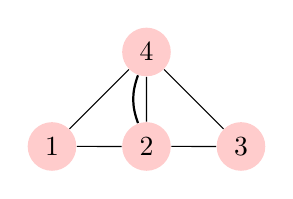
\begin{tikzpicture}
  [scale=.6,auto=left,every node/.style={circle,fill=red!20}]
  \node (n1) at (1,7) {1};
  \node (n2) at (3,7)  {2};
  \node (n3) at (5,7)  {3};
  \node (n4) at (3,9)  {4};

  \foreach \from/\to in {n1/n2,n2/n3,n2/n4,n1/n4,n3/n4}
    \draw (\from) -- (\to);
\path[thick] (n2) edge[bend left=20] (n4);
\end{tikzpicture}
\caption{ Graph in Figure \ref{4g1} with edge (2,4) added to have a closed Eulerian Walk}\label{4g155}
\end{center}
\end{figure}

\vspace{3in}
Rishnak asked Ajur whether he knew about multi graphs and directed graphs. Ajur realized he essentially learnt about multigraphs  by doing Eulerian walks and completion  example. Ajur added that in a direct an edge $(x,y)$ goes from vertex $x$ to $y$ and he drew an example graph to show Rishnak that he knows See Figure \ref{4g5}. Ajur added that instead of degree of a vertex, we have in-degree and out-degree of a vertex. The number of edges coming to a vertex is the in-degree of that vertex and the number of edges going out of a vertex is the out-degree of a vertex,
\begin{figure}
\begin{center}
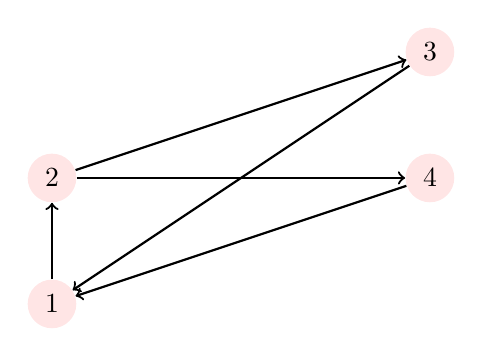
\begin{tikzpicture}
  [scale=.8,auto=left,every node/.style={circle,fill=red!10}]
  \node (n1) at (1,7) {1};
  \node (n2) at (1,9)  {2};
  \node (n3) at (7,11)  {3};
  \node (n4) at (7,9) {4};
 \path[->, draw,thick] 
        (n1) edge (n2)
         (n3) edge (n1)
        (n2) edge (n3)
        (n2) edge (n4)
        (n4) edge  (n1);

\end{tikzpicture}
\caption{ Example Directed Graph with 4 vertices and 5 edges}\label{4g5}
\end{center}
\end{figure}

Anticipating what Rishnak is going to ask, 